%-------------------------------------------------------------------------------
\section{Introduction}
\label{s:intro}
%-------------------------------------------------------------------------------

Many microservices are \textit{latency critical} (LC), meaning that the people
running them care about their response time. When latency critical applications
take significantly longer than expected to process requests, bad things happen:
customers are turned off, and revenue is lost~\cite{google-speed-matters,
amz-speed-matters}.\hmng{might be helpful to give a sense of the time scale we
are targeting} In order to give developers a predictable environment for
critical services to run in, providers expose an interface for reserving
resources: developers using platforms like AWS ec2 or Kubernetes attach to each
service they want to run a fixed amount of resources the service will get, \ie{}
a number of CPUs and an amount of memory~\cite{aws-ec2-resources,
kubernetes-resources}. The guarantee developers get is that the service will
have undisturbed access to that amount of resources.

However, this leads to a utilization problem for providers. The load on the
microservices is usually variable and unpredictable, so to account for this
developers choose the amount of resources to reserve based on the expected peak
load~\cite{borg, nu, overprovision}. This means that LC services rarely use the
full resource reservation they asked for.

\textit{Best effort} (BE) tasks, on the other hand, are tasks whose completion
time is not critical. Popular examples include long-running map reduce jobs or
background data analytics. Many cloud scheduling systems support LC and BE
tasks; this includes distributed schedulers, \eg{} Borg\cite{borg} or
Kubernetes\cite{kubernetes-resources}, and single machine schedulers, for
example Caladan\cite{caladan}.

Running BE alongside LC helps providers solve the utilization problem caused by
overprovisioning on the part of LCs. BE tasks can run on unused resources
opportunistically, because they can tolerate delays when LC load spikes. In
order do so while guaranteeing LC services predictable and uncontended access to
the resources they reserved, the platform needs to maintain strict isolation
between the two. BEs share all the hardware resources with the LC, and LCs need
isolation on all of them. The resource that this work focuses on is CPU.


\begin{figure}[t]
    \centering
    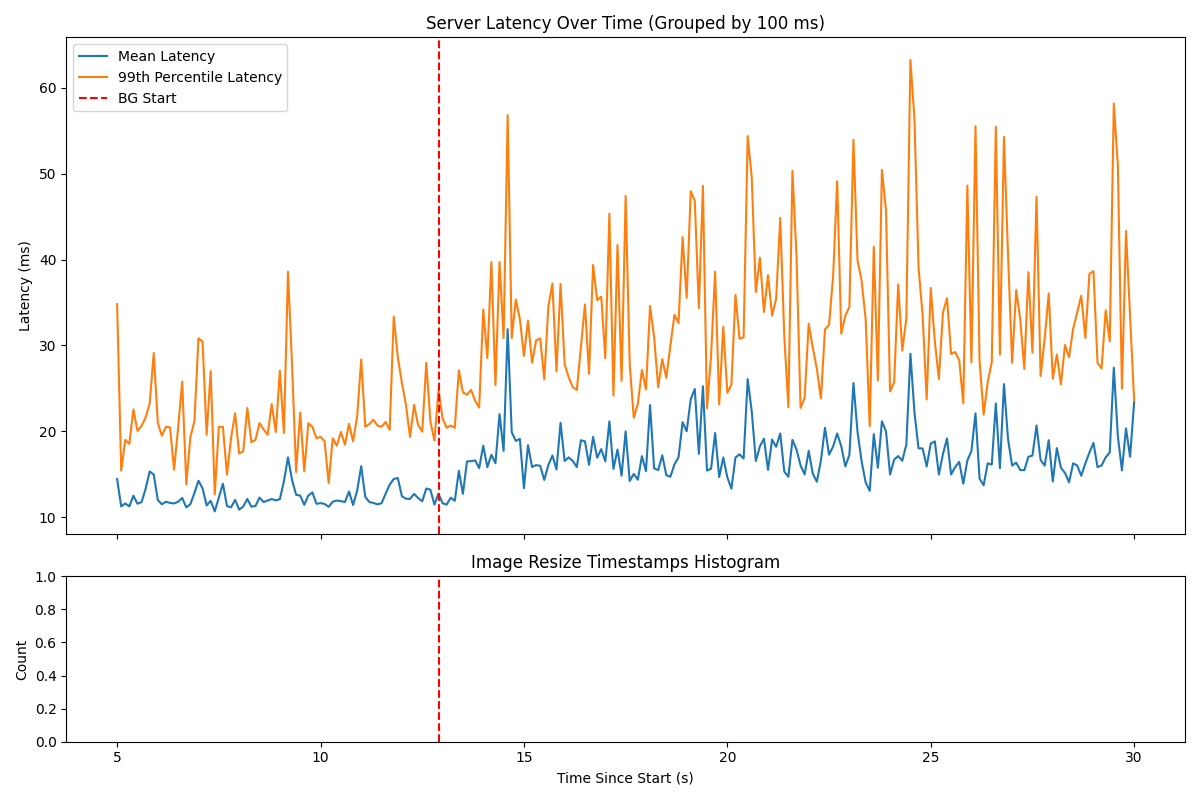
\includegraphics[width=\columnwidth]{graphs/kubernetes-unedited.png}
    \caption{E2E repsonse times for a simple social network web application,
    before and after starting load on a BE service; Kubernetes allows BE to
    interfere with LC}\label{fig:kubernetes-unedited}
\end{figure}

We find that current popular scheduling systems fail to properly isolate latency
critical from best effort workloads. When running a small but realistic social
network web application on Kubernetes, we observe significant impacts on its
latency when starting a best effort workload, doing image resizing, on the same
machine. The top graph of \autoref{fig:kubernetes-unedited} plots the end-to-end
latency of an endpoint that gets a users feed and applies a moderation; the
bottom graph shows the throughput of the BE workload. After the BEs start
running, the mean response latency of the web application jumps from $\sim$7ms
to $\sim$15ms, and the 99th percentile latency from $\sim$10ms to $\sim$25ms. 

Understanding where the isolation fails requires looking at the underlying
mechanism that is enforcing it: Linux's \cgroups{}. Most modern containers rely
on \cgroups{} for CPU isolation; this includes all Open Container Initiative
(OCI) compliant containers, including Kubernetes but also Docker, CRI-O, and
containerd~\cite{oci-cgroups,docker-docs-cgroups,container-isolation-article}.
VM frameworks, including Firecracker, AFaas and libvirt, also rely on \cgroups{}
to manage CPU time allocation when the number of vCPUs is
oversubscribed.~\cite{firecracker-cgroups,afaas,libvirt-cgroups}

The part of the \cgroups{} interface that these systems use to isolate LC and BE
is based on weight.\footnote{Other operating systems expose a similar interface,
for instance Windows exposes a number of shares.} Kubernetes creates one top
level group for all BEs, \texttt{kubepods-besteffort}, inside which all BE pods
are placed, and assigns it the lowest possible weight of 1. LC pods are
separated into Burstable and Guaranteed, the main difference being that
Guaranteed pods require a limit to be set on the resources it can use.
Kubernetes calculates the weight that each pod gets based on the amount of
milliCPUs they request. For instance, in the \autoref{fig:kubernetes-unedited}
experiment, the LC service ran in the Guaranteed class and asked for 4 CPUs, and
was assigned a weight of 157. 

\cgroups{} specifies that each group should get CPU time proportional to its
weight as a share of the sum of weights of runnable
groups~\cite{cgroups-kerneldocs}. However, we can see that this is not true for
the application in \autoref{fig:kubernetes-unedited}. As we show in more detail
in \autoref{s:problem}, the problem that leads to the increased latencies
observed is that Linux will run a BE process on one core, unaware that an LC
process is runnable and waiting on another. This happens because Linux uses
per-CPU runqueues, which avoids the overheads of having a global runqueue. A key
challenge this work addresses is how to manage this tension between expensive
cross-core checks and affecting strict isolation across cores.

Our approach addresses this challenge by exposing in the API a new priority
class for BE to run in, \beclass{}, and enforcing it in the scheduler via strict
priority scheduling. As we show in \autoref{ss:approach:solves-problems},
putting BE in a separate class from LC makes it viable to enforce the isolation
across cores, because it reduces the number of times the scheduler is required
to look at other runqueues. Enforcing weights across cores requires the
scheduler to do so every scheduling tick, but with a separate class it only has
to look at other cores on \textit{class boundary crossings}: every time a core
swtiches from an LC to running a BE process, and every time it queues an LC one.

A challenge that emerges from creating a separate priority class is that, when
the LC is under high load, completely starving BE processes can lead to issues
such as broken TCP connections or missed timers. The goal is to make the
priority of LC over BE as strict as possible, while allowing BE processes to
resume execution normally once the load goes down, even if the high load lasts
for multiple minutes.

We address this challenge by enabling BEs to exist in an ephemeral state called
\textit{parked}, which BEs enter when the CPU utilization is high enough that
any amount of running a BE would interfere with an LC. While load remains high,
the scheduler ensures that the user-space process doesn't run and consume
resources, but continues to run the kernel-space handlers that manage critical
state, including TCP connections and timers, on behalf of the BE processes. 

Linux has classes between which it enforces strict priority, but those are
designed and used for real time applications, and use scheduling algorithms
within the classes that are not well-suited for microservice applications. We
discuss them in \autoref{s:existing}, and motivate \beclass{} as a new
scheduling class that sits below the default scheduling class running LCs.

We implement \beclass{} in Linux, and show that it is able to significiantly
improve Linux's ability to isolate LC from BE workloads: in the same Kubernetes
experiment, the increase in average latency when starting a BE workload goes
from $>$2x to 0. The contributions of this paper are thus as follows: 
\begin{enumerate}
    \item identifying as the reason isolation between LC and BE often fails that
    \cgroups{} does a poor job of enforcing the weights across cores; and that
    this dramatically affects end-to-end latencies
    \item the design of \beclass{}, a new class for BE tasks that separates
    them from the default class LC tasks run in, and isolates LC workloads from
    BE ones while minimizing the amount of cross-core checks required, as well as
    naturally enforcing the parked state
    \item an implementation of \beclass{} in Linux
\end{enumerate}
